\documentclass[prb,singlecolumn]{revtex4}

\usepackage{amssymb}
\usepackage{amsmath}
\usepackage{amsfonts}
\usepackage{amsbsy}
\newcommand{\Eqref}[1]{Eq.~(\ref{#1})}
\newcommand{\Fref}[1]{Fig.~\ref{#1}}
\newcommand{\alf}{{Alfv\'en~}}

\usepackage{tikz}
\usetikzlibrary{decorations.pathreplacing,decorations.pathmorphing}

\begin{document}


\title{Self-sustained turbulence in magnetized shear flow}
\author{Zlatan D.~Dimitrov}
\email{zlatan.dimitrov@}
\author{Todor M.~Mishonov}
\email{tmishonov@phys.}
\affiliation{Department of Theoretical Physics, Faculty of Physics,\\
University of Sofia St.~Clement of Ohrid,\\
5 J. Bourchier Blvd, BG-1164 Sofia, Bulgaria}

\date{\today}

\maketitle

\begin{eqnarray}
\mathrm{D}_{\overline{\tau}}^{\mathrm{\,shear}}\mathbf{v}_\mathbf{Q}(\tau) &=&
-v_{x,\mathbf{Q}}\mathbf{e}_y + 2n_y\mathbf{n}v_{x,\mathbf{Q}}
-\nu^\prime_\mathrm{k}Q^2\mathbf{v}_\mathbf{Q} + \Pi^{\perp\mathbf{Q}}\cdot\sum_{\mathbf{Q}'}\left[\mathbf{v}_{\mathbf{Q}'}\otimes\mathbf{v}_{\mathbf{Q}
-\mathbf{Q}'} + \mathbf{b}_{\mathbf{Q}'}\otimes\mathbf{b}_{\mathbf{Q}-\mathbf{Q}'}\right]\cdot\mathbf{Q},
\label{VelocityEvolution}
\\
\label{MagneticEvolution}
\mathrm{D}_{\overline{\tau}}^{\mathrm{\,shear}}\mathbf{b}_\mathbf{Q}(\tau) &=& b_{x,\mathbf{Q}}\mathbf{e}_y
-(\mathbf{Q}\cdot{\alpha})\,\mathbf{v}_\mathbf{Q} -\nu'_\mathrm{m}Q^2\mathbf{b}_\mathbf{Q} + \Pi^{\perp\mathbf{Q}}\cdot\sum_{\mathbf{Q}'}\left[\mathbf{b}_{\mathbf{Q}'}\otimes\mathbf{v}_{\mathbf{Q}
-\mathbf{Q}'} - \mathbf{v}_{\mathbf{Q}'}\otimes\mathbf{b}_{\mathbf{Q}-\mathbf{Q}'}\right]\cdot\mathbf{Q}, 
\\
\mathbf{Q} \cdot \mathbf{N}_v &=& 0, \quad \mathbf{v}_\mathbf{Q}(\overline{\tau}_0)=\Pi^{\perp\mathbf{Q}}\mathbf{v}_\mathbf{Q}(\overline{\tau}_0),\quad
\mathbf{Q}\cdot \mathbf{N}_b=0, \quad \mathbf{b}_\mathbf{Q}(\overline{\tau}_0)=\Pi^{\perp\mathbf{Q}}\mathbf{b}_\mathbf{Q}(\overline{\tau}_0),\nonumber 
\\
\Pi^{\perp\mathbf{Q}} &\equiv &\openone-\mathbf{n}\otimes \mathbf{n},\quad \mathbf{n}\equiv \frac{\mathbf{Q}}{Q},\quad \overline{\tau}\equiv-\frac{Q_x}{Q_y}
\\
\label{ushear}
\mathrm{D}_\tau^{\mathrm{\,shear}} &\equiv& \partial_\tau+\mathbf{U}_{\mathrm{shear}}(\mathbf{Q})\cdot\partial_{\mathbf{Q}}=\partial_\tau-Q_y\partial_{Q_x}= \partial_\tau + \partial_{\overline{\tau}},\quad
\mathbf{U}_\mathrm{shear}(\mathbf{Q})\equiv-Q_y\mathbf{e}_x, 
\end{eqnarray}

\begin{eqnarray}
 \mathrm{d}_{\overline{\tau}}\, v_y &=& -v_x + 2 n_y^2 v_x + Q_yb_y - \nu^\prime_\mathrm{k}Q^2v_y + N_v^y, \\
 \mathrm{d}_{\overline{\tau}}\, b_y &=& b_x  -Q_yv_y -\nu^\prime_\mathrm{m}Q^2b_y + N_b^y.
\end{eqnarray}


\begin{equation}
\label{bay_ivan}
\mathrm{d}^2_{\overline{\tau}}b_y + \nu_\mathrm{tot}^\prime Q^2\mathrm{d}_{\overline{\tau}}b_y + [Q^2_\alpha + 2\nu_\mathrm{m}^\prime \overline{\tau} Q_y^2 +\nu_\mathrm{m}^\prime\nu_\mathrm{k}^\prime Q^4]b_y
= \mathrm{d}_{\overline{\tau}}N^y_b - Q_\alpha N_v^y -2Q_\alpha n_y^2v_x + \nu_\mathrm{k}^\prime QN_b^y + (\nu_\mathrm{k}^\prime - \nu_\mathrm{m}^\prime)b_x.
\end{equation}


\begin{equation}
\lim\limits_{\nu'_\mathrm{k} \rightarrow 0}{\left(\frac{\int_0^\infty\nu'_\mathrm{k}\overline{\tau}^2e^{-\nu'_\mathrm{tot} Q_y^2\overline{\tau}^2/6}\mathrm{d}\overline{\tau}}{\int_0^\infty e^{-\nu'_\mathrm{tot} Q_y^2\overline{\tau}^2/6}\mathrm{d}\overline{\tau}} = \frac{6^{2/3}}{3\Gamma(\frac43)} \frac{\nu_\mathrm{k}^{_\prime 1/3}}{Q_y^{4/3}(1+\frac{1}{\mathrm{P}_\mathrm{m}})^{2/3} }\right)} = 0.
\end{equation}

\begin{equation}
\left[ \mathrm{d}^2_{\overline{\tau}} + \nu_\mathrm{tot}^\prime Q^2\mathrm{d}_{\overline{\tau}} + Q^2_\alpha \right]b_y =
\mathrm{d}_{\overline{\tau}}N^y_b - Q_\alpha N_v^y.
\end{equation}


\begin{eqnarray}
\mathbf{N}_v  = \Pi^{\perp\mathbf{Q}}\cdot\sum_{\mathbf{Q}'}
\left[
\left(\begin{array}{ccc}
v_{\mathbf{Q}'}^xv_{\mathbf{Q}-\mathbf{Q}'}^x & v_{\mathbf{Q}'}^xv_{\mathbf{Q}-\mathbf{Q}'}^y & v_{\mathbf{Q}'}^xv_{\mathbf{Q}-\mathbf{Q}'}^z \\
v_{\mathbf{Q}'}^yv_{\mathbf{Q}-\mathbf{Q}'}^x & v_{\mathbf{Q}'}^yv_{\mathbf{Q}-\mathbf{Q}'}^y & v_{\mathbf{Q}'}^yv_{\mathbf{Q}-\mathbf{Q}'}^z \\
v_{\mathbf{Q}'}^zv_{\mathbf{Q}-\mathbf{Q}'}^x & v_{\mathbf{Q}'}^zv_{\mathbf{Q}-\mathbf{Q}'}^y & v_{\mathbf{Q}'}^zv_{\mathbf{Q}-\mathbf{Q}'}^z
\end{array} \right)
+
\left(\begin{array}{ccc}
b_{\mathbf{Q}'}^xb_{\mathbf{Q}-\mathbf{Q}'}^x & b_{\mathbf{Q}'}^xb_{\mathbf{Q}-\mathbf{Q}'}^y & b_{\mathbf{Q}'}^xb_{\mathbf{Q}-\mathbf{Q}'}^z \\
b_{\mathbf{Q}'}^yb_{\mathbf{Q}-\mathbf{Q}'}^x & b_{\mathbf{Q}'}^yb_{\mathbf{Q}-\mathbf{Q}'}^y & b_{\mathbf{Q}'}^yb_{\mathbf{Q}-\mathbf{Q}'}^z \\
b_{\mathbf{Q}'}^zb_{\mathbf{Q}-\mathbf{Q}'}^x & b_{\mathbf{Q}'}^zb_{\mathbf{Q}-\mathbf{Q}'}^y & b_{\mathbf{Q}'}^zb_{\mathbf{Q}-\mathbf{Q}'}^z
\end{array} \right)
\right]
\cdot
\left(\begin{array}{c}
Q_x \\
Q_y \\
Q_z
\end{array} \right),
\end{eqnarray}

\begin{eqnarray}
\mathbf{N}_b  = \Pi^{\perp\mathbf{Q}}\cdot\sum_{\mathbf{Q}'}
\left[
\left(\begin{array}{ccc}
b_{\mathbf{Q}'}^xv_{\mathbf{Q}-\mathbf{Q}'}^x & b_{\mathbf{Q}'}^xv_{\mathbf{Q}-\mathbf{Q}'}^y & b_{\mathbf{Q}'}^xv_{\mathbf{Q}-\mathbf{Q}'}^z \\
b_{\mathbf{Q}'}^yv_{\mathbf{Q}-\mathbf{Q}'}^x & b_{\mathbf{Q}'}^yv_{\mathbf{Q}-\mathbf{Q}'}^y & b_{\mathbf{Q}'}^yv_{\mathbf{Q}-\mathbf{Q}'}^z \\
b_{\mathbf{Q}'}^zv_{\mathbf{Q}-\mathbf{Q}'}^x & b_{\mathbf{Q}'}^zv_{\mathbf{Q}-\mathbf{Q}'}^y & b_{\mathbf{Q}'}^zv_{\mathbf{Q}-\mathbf{Q}'}^z
\end{array} \right)
-
\left(\begin{array}{ccc}
v_{\mathbf{Q}'}^xb_{\mathbf{Q}-\mathbf{Q}'}^x & v_{\mathbf{Q}'}^xb_{\mathbf{Q}-\mathbf{Q}'}^y & v_{\mathbf{Q}'}^xb_{\mathbf{Q}-\mathbf{Q}'}^z \\
v_{\mathbf{Q}'}^yb_{\mathbf{Q}-\mathbf{Q}'}^x & v_{\mathbf{Q}'}^yb_{\mathbf{Q}-\mathbf{Q}'}^y & v_{\mathbf{Q}'}^yb_{\mathbf{Q}-\mathbf{Q}'}^z \\
v_{\mathbf{Q}'}^zb_{\mathbf{Q}-\mathbf{Q}'}^x & v_{\mathbf{Q}'}^zb_{\mathbf{Q}-\mathbf{Q}'}^y & v_{\mathbf{Q}'}^zb_{\mathbf{Q}-\mathbf{Q}'}^z
\end{array} \right)
\right]
\cdot
\left(\begin{array}{c}
Q_x \\
Q_y \\
Q_z
\end{array} \right),
\end{eqnarray}


$\Pi^{\perp\mathbf{Q}}$ is the projection operator and have

\begin{eqnarray}
\lim\limits_{\tau \rightarrow \infty}{ \Pi^{\perp\mathbf{Q}} } = \left(\begin{array}{ccc}
 0 & 0 & 0 \\
 0 & 1 & 0 \\
 0 & 0 & 1 
\end{array} \right)
\end{eqnarray}



\begin{eqnarray}
 \lim\limits_{\tau \rightarrow \infty}{\mathbf{N}_b} &=&
\left(\begin{array}{c}
 0  \\
 \sum_{\mathbf{Q}'} (b_{\mathbf{Q}'}^yv_{\mathbf{Q}-\mathbf{Q}'}^y - v_{\mathbf{Q}'}^yb_{\mathbf{Q}-\mathbf{Q}'}^y)Q_y + (b_{\mathbf{Q}'}^yv_{\mathbf{Q}-\mathbf{Q}'}^z - v_{\mathbf{Q}'}^yb_{\mathbf{Q}-\mathbf{Q}'}^z)Q_z  \\
 \sum_{\mathbf{Q}'} (b_{\mathbf{Q}'}^zv_{\mathbf{Q}-\mathbf{Q}'}^y - v_{\mathbf{Q}'}^zb_{\mathbf{Q}-\mathbf{Q}'}^y)Q_y + (b_{\mathbf{Q}'}^zv_{\mathbf{Q}-\mathbf{Q}'}^z - v_{\mathbf{Q}'}^zb_{\mathbf{Q}-\mathbf{Q}'}^z)Q_z \end{array} \right) \\
  \lim\limits_{\tau \rightarrow \infty}{\mathbf{N}_v} &=&
\left(\begin{array}{c}
 0  \\
 \sum_{\mathbf{Q}'} (v_{\mathbf{Q}'}^yv_{\mathbf{Q}-\mathbf{Q}'}^y + b_{\mathbf{Q}'}^yb_{\mathbf{Q}-\mathbf{Q}'}^y)Q_y + (v_{\mathbf{Q}'}^yv_{\mathbf{Q}-\mathbf{Q}'}^z + b_{\mathbf{Q}'}^yb_{\mathbf{Q}-\mathbf{Q}'}^z)Q_z \\
 \sum_{\mathbf{Q}'} (v_{\mathbf{Q}'}^zv_{\mathbf{Q}-\mathbf{Q}'}^y + b_{\mathbf{Q}'}^zb_{\mathbf{Q}-\mathbf{Q}'}^y)Q_y + (v_{\mathbf{Q}'}^zv_{\mathbf{Q}-\mathbf{Q}'}^z + b_{\mathbf{Q}'}^zb_{\mathbf{Q}-\mathbf{Q}'}^z)Q_z \end{array} \right)
\end{eqnarray}


\begin{eqnarray*}
&&\mathrm{d}_{\overline{\tau}}N_b^y = \mathrm{d}_{\overline{\tau}}\left[\sum_{\mathbf{Q}'} (b_{\mathbf{Q}'}^yv_{\mathbf{Q}-\mathbf{Q}'}^y - v_{\mathbf{Q}'}^yb_{\mathbf{Q}-\mathbf{Q}'}^y)Q_y + (b_{\mathbf{Q}'}^yv_{\mathbf{Q}-\mathbf{Q}'}^z - v_{\mathbf{Q}'}^yb_{\mathbf{Q}-\mathbf{Q}'}^z)Q_z \right] \\
&& =\sum_{\mathbf{Q}'} [(b_{\mathbf{Q}'}^yb_{\mathbf{Q}-\mathbf{Q}'}^y + v_{\mathbf{Q}'}^yv_{\mathbf{Q}-\mathbf{Q}'}^y)Q_y + (b_{\mathbf{Q}'}^yb_{\mathbf{Q}-\mathbf{Q}'}^z + v_{\mathbf{Q}'}^yv_{\mathbf{Q}-\mathbf{Q}'}^z)Q_z](Q_y-Q'_y) ,  \\
&&\mathrm{d}_{\overline{\tau}} v_{\mathbf{Q}-\mathbf{Q}'}^y = (Q_y-Q'_y)b_{\mathbf{Q}-\mathbf{Q}'}^y,\quad \mathrm{d}_{\overline{\tau}} b_{\mathbf{Q}-\mathbf{Q}'}^y = -(Q_y-Q'_y)v_{\mathbf{Q}-\mathbf{Q}'}^y \nonumber
\end{eqnarray*}
  
For the resulting external force acting on the out oscillator we have
%
\begin{eqnarray}
&&F_\mathrm{ext} =\mathrm{d}_{\overline{\tau}}N_b^y - Q_yN_v^y=\nonumber \\
&&\sum_{\mathbf{Q}'}\left\{ \left[(b_{\mathbf{Q}'}^yb_{\mathbf{Q}-\mathbf{Q}'}^y + v_{\mathbf{Q}'}^yv_{\mathbf{Q}-\mathbf{Q}'}^y)Q_y + (b_{\mathbf{Q}'}^yb_{\mathbf{Q}-\mathbf{Q}'}^z + v_{\mathbf{Q}'}^yv_{\mathbf{Q}-\mathbf{Q}'}^z)Q_z\right](Q_y-Q'_y)\right\} -\\
&&\sum_{\mathbf{Q}'}\left\{ \left[(b_{\mathbf{Q}'}^yb_{\mathbf{Q}-\mathbf{Q}'}^y + v_{\mathbf{Q}'}^yv_{\mathbf{Q}-\mathbf{Q}'}^y)Q_y + (b_{\mathbf{Q}'}^yb_{\mathbf{Q}-\mathbf{Q}'}^z + v_{\mathbf{Q}'}^yv_{\mathbf{Q}-\mathbf{Q}'}^z)Q_z\right](-Q_y)\right\}=\\
&&-\sum_{\mathbf{Q}'}\left\{ \left[(b_{\mathbf{Q}'}^yb_{\mathbf{Q}-\mathbf{Q}'}^y + v_{\mathbf{Q}'}^yv_{\mathbf{Q}-\mathbf{Q}'}^y)Q_y + (b_{\mathbf{Q}'}^yb_{\mathbf{Q}-\mathbf{Q}'}^z + v_{\mathbf{Q}'}^yv_{\mathbf{Q}-\mathbf{Q}'}^z)Q_z\right]Q'_y\right\}
\end{eqnarray}



\begin{eqnarray}
b_y(\overline{\tau},Q_y,Q_z) &=&
\int_{-\infty}^{\overline{\tau}} \mathrm{d}\overline{\tau_0} \frac{\sin[Q_y(\overline{\tau}-\overline{\tau}_0)]}{Q_y}
\exp\left(-\frac12\int^{\overline{\tau}}_{\overline{\tau}_0} \nu^\prime_\mathrm{tot} Q^2(\tau) \mathrm{d}\tau \right) \theta(\overline{\tau}-\overline{\tau}_0) F_\mathrm{ext}(\overline{\tau}_0)=\\
&&= \sin(Q_y\overline{\tau}) \int^{\overline{\tau}}_{-\infty}\mathrm{d}\overline{\tau_0} \frac1{Q_y}\cos(Q_y\overline{\tau_0})\exp\left[ -\frac{\nu^{\prime}_{\mathrm{tot}}}{6}(\overline{\tau}^3 - \overline{\tau_0}^3)Q_y^2 \right]  F_\mathrm{ext}(\overline{\tau}_0) \nonumber \\
&& - \cos(Q_y\overline{\tau}) \int^{\overline{\tau}}_{-\infty}\mathrm{d}\overline{\tau_0} \frac1{Q_y}\sin(Q_y\overline{\tau_0})\exp\left[ -\frac{\nu^{\prime}_{\mathrm{tot}}}{6}(\overline{\tau}^3 - \overline{\tau_0}^3)Q_y^2 \right]  F_\mathrm{ext}(\overline{\tau}_0) \nonumber
\end{eqnarray}

\begin{eqnarray}
 X(\overline{\tau},Q_y,Q_z) &=& \int^{\overline{\tau}}_{-\infty}\mathrm{d}\overline{\tau_0} \frac1{Q_y}\cos(Q_y\overline{\tau_0})\exp\left[ -\frac{\nu^{\prime}_{\mathrm{tot}}}{6}(\overline{\tau}^3 - \overline{\tau_0}^3)Q_y^2 \right]  F_\mathrm{ext}(\overline{\tau}_0) \nonumber \\
 Y(\overline{\tau},Q_y,Q_z) &=& - \int^{\overline{\tau}}_{-\infty}\mathrm{d}\overline{\tau_0} \frac1{Q_y}\sin(Q_y\overline{\tau_0})\exp\left[ -\frac{\nu^{\prime}_{\mathrm{tot}}}{6}(\overline{\tau}^3 - \overline{\tau_0}^3)Q_y^2 \right]  F_\mathrm{ext}(\overline{\tau}_0) \nonumber 
\end{eqnarray}

\begin{equation}
 b_y(\overline{\tau},Q_y,Q_z)  =\sin(Q_y\overline{\tau})X(\overline{\tau}) + \cos(Q_y\overline{\tau})Y(\overline{\tau}) \approx X_0 \cos(Q_y\overline{\tau}) + Y_0\sin(Q_y\overline{\tau})
\end{equation}


\begin{eqnarray}
b_z(\xi) &=& \frac{2K_z}{K_\perp} \int_{-\infty}^{\xi} \frac{\sin\left[K_\perp(\xi-\xi^\prime) \right]}{K_\perp(1+\xi^\prime)^{5/2}}
 \left[ (1+\xi'^2)\mathrm{d}_{\xi'}\psi(\xi') - \xi'\psi(\xi') \right] \mathrm{d}\xi' = \\
&& \frac{2K_z\sin(K_\perp\xi)}{K_\perp} \int_{-\infty}^{\xi} \frac{\cos\left(K_\perp\xi^\prime \right)}{K_\perp(1+\xi^\prime)^{5/2}}
 \left[ (1+\xi'^2)\left(C_\mathrm{g}\mathrm{d}_{\xi'}\psi_\mathrm{g}(\xi') + C_\mathrm{u}\mathrm{d}_{\xi'}\psi_\mathrm{u}(\xi') \right)- \xi'\left(C_\mathrm{g}\psi_\mathrm{g}(\xi') + C_\mathrm{u}\psi_\mathrm{u}(\xi') \right)  \right] \mathrm{d}\xi' \nonumber
 - \\
&& \frac{2K_z\cos(K_\perp\xi)}{K_\perp} \int_{-\infty}^{\xi} \frac{\sin\left(K_\perp\xi^\prime \right)}{K_\perp(1+\xi^\prime)^{5/2}}
 \left[ (1+\xi'^2)\left(C_\mathrm{g}\mathrm{d}_{\xi'}\psi_\mathrm{g}(\xi') + C_\mathrm{u}\mathrm{d}_{\xi'}\psi_\mathrm{u}(\xi') \right)- \xi'\left(C_\mathrm{g}\psi_\mathrm{g}(\xi') + C_\mathrm{u}\psi_\mathrm{u}(\xi') \right) \right] \mathrm{d}\xi' \nonumber
 = \\
&& \frac{2K_z}{K_\perp}\left[ J_{c,\mathrm{u}}C_\mathrm{u}\sin(K_\perp\xi)  - J_{s,\mathrm{g}}C_\mathrm{g}\cos(K_\perp\xi) \right] \approx \frac{4K_z}{K_\perp^2}C_\mathrm{u}\sin(K_\perp\xi) + \frac{4K_z}{3K_\perp}C_\mathrm{g}\cos(K_\perp\xi), \nonumber
\\
&& 
J_{c,\mathrm{u}} = \int_{-\infty}^{\infty} \frac{\cos\left(K_\perp\xi^\prime \right)}{K_\perp(1+\xi^\prime)^{5/2}} \left[ (1+\xi'^2)\left(C_\mathrm{u}\mathrm{d}_{\xi'}\psi_\mathrm{u}(\xi') \right)- \xi' C_\mathrm{u}\psi_\mathrm{u}(\xi') \right], \lim_{K_\perp \rightarrow 0} J_{c,\mathrm{u}} = \frac2{K_\perp}\nonumber \\ 
&&
J_{s,\mathrm{g}} = \int_{-\infty}^{\infty} \frac{\sin\left(K_\perp\xi^\prime \right)}{K_\perp(1+\xi^\prime)^{5/2}} \left[ (1+\xi'^2)\left(C_\mathrm{g}\mathrm{d}_{\xi'}\psi_\mathrm{g}(\xi') \right)- \xi' C_\mathrm{g}\psi_\mathrm{g}(\xi') \right], \lim_{K_\perp \rightarrow 0} J_{c,\mathrm{u}} = -\frac23 \nonumber \\
v_z(\xi) &=& \frac{2K_z}{K_\perp} \int_{-\infty}^{\xi} \frac{\cos\left[K_\perp(\xi-\xi^\prime) \right]}{K_\perp(1+\xi^\prime)^{5/2}}
 \left[ (1+\xi'^2)\mathrm{d}_{\xi'}\psi(\xi') - \xi'\psi(\xi') \right] \mathrm{d}\xi' = \nonumber \\
&& \frac{2K_z\cos(K_\perp\xi)}{K_\perp} \int_{-\infty}^{\xi} \frac{\cos\left(K_\perp\xi^\prime \right)}{K_\perp(1+\xi^\prime)^{5/2}}
 \left[ (1+\xi'^2)C_\mathrm{u}\mathrm{d}_{\xi'}\psi_\mathrm{u}(\xi') - \xi'C_\mathrm{u}\psi_\mathrm{u}(\xi')  \right] \mathrm{d}\xi' \nonumber
 + \\
&& \frac{2K_z\sin(K_\perp\xi)}{K_\perp} \int_{-\infty}^{\xi} \frac{\sin\left(K_\perp\xi^\prime \right)}{K_\perp(1+\xi^\prime)^{5/2}}
 \left[ (1+\xi'^2)C_\mathrm{g}\mathrm{d}_{\xi'}\psi_\mathrm{g}(\xi') - \xi'C_\mathrm{g}\psi_\mathrm{g}(\xi') \right] \mathrm{d}\xi' \nonumber
 = \\
&& \frac{2K_z}{K_\perp}\left[ J_{c,\mathrm{u}}C_\mathrm{u}\cos(K_\perp\xi)  - J_{s,\mathrm{g}}C_\mathrm{g}\sin(K_\perp\xi) \right] \approx \frac{4K_z}{K_\perp^2}C_\mathrm{u}\cos(K_\perp\xi) + \frac{4K_z}{3K_\perp}C_\mathrm{g}\sin(K_\perp\xi) \nonumber \\
b_y &=& -\frac{2K_z^2}{K_\perp K_y} [\sin(K_\perp\xi) I_c(\xi) - \cos(K_\perp\xi) I_s(\xi)] + \frac{K_\perp}{K_y}\frac{\xi\psi(\xi)}{\sqrt{1+\xi^2}} \approx -\frac{4K_z^2}{K_\perp^2 K_y}C_\mathrm{u}\sin(K_\perp\xi) - \frac{4K_z^2}{K_\perp K_y}C_\mathrm{g}\cos(K_\perp\xi) + \frac{K_\perp}{K_y}\psi(\xi) \nonumber \\
v_y &=& -\frac{2K_z^2}{K_\perp K_y} [\cos(K_\perp\xi) I_c(\xi) - \sin(K_\perp\xi) I_s(\xi)] + \frac{\mathrm{d}_\xi \psi(\xi)}{K_y} \approx -\frac{4K_z^2}{K_\perp^2 K_y}C_\mathrm{u}\cos(K_\perp\xi) - \frac{4K_z^2}{K_\perp K_y}C_\mathrm{g}\sin(K_\perp\xi) + \frac{\mathrm{d}_\xi \psi(\xi)}{K_y} \nonumber
\end{eqnarray}

\begin{figure}
  \centering
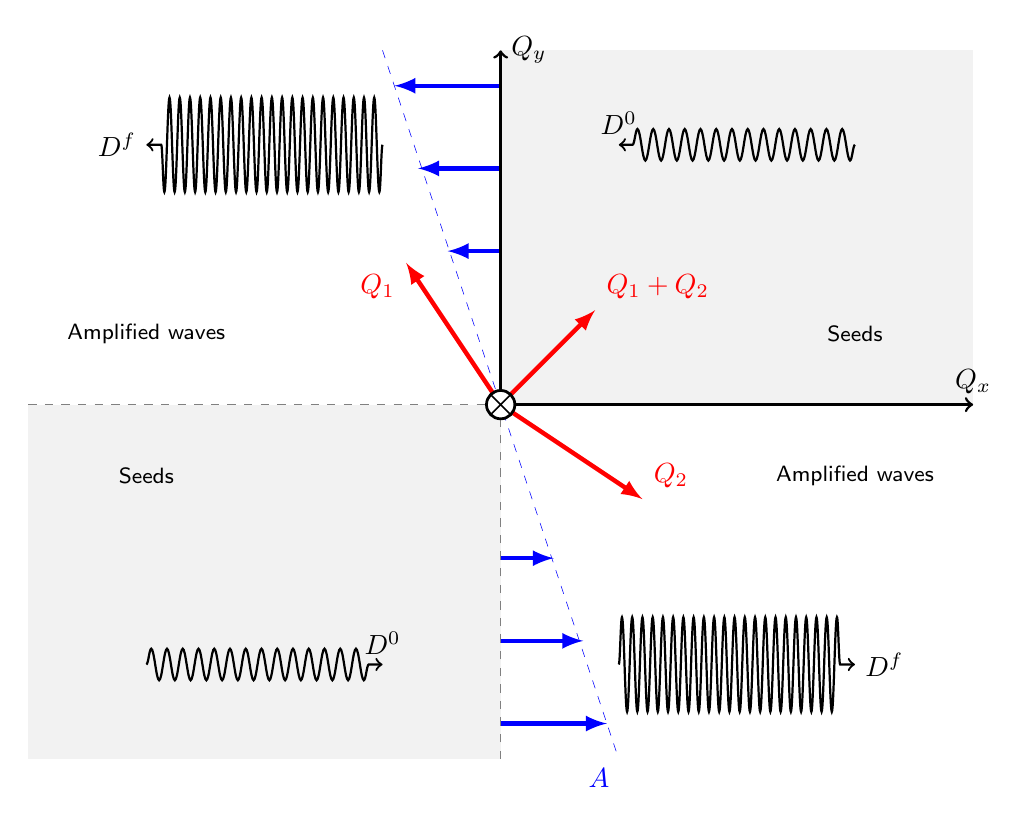
\begin{tikzpicture}[
    media/.style={font={\footnotesize\sffamily}},
    wave/.style={decorate,decoration={snake,post length=1.4mm,amplitude=2mm, segment length=2mm},thick},
    awave/.style={decorate,decoration={snake,post length=1.4mm,amplitude=6mm, segment length=1.3mm},thick},
    interface/.style={ postaction={draw,decorate,decoration={border,angle=-45, amplitude=0.3cm,segment length=2mm}}},
    scale=1.5]

    \fill[gray!10] (0,3) rectangle (4,0);
    \fill[gray!10] (-4,-3) rectangle (0,0);

     \draw[dashed,gray](0,-3)--(0,3);
     \draw[dashed,gray](-4,0)--(4,0);

     \coordinate (Origin)   at (0,0);

    \coordinate (Bone) at (-0.8,1.2);
    \coordinate (Btwo) at (1.2,-0.8);

    \draw [ultra thick,-latex,red] (Origin) -- (Bone) node [below left] {$Q_1$};
    \draw [ultra thick,-latex,red] (Origin) -- (Btwo) node [above right] {$Q_2$};
    \draw [ultra thick,-latex,red] (Origin) -- (0.8,0.8) node [above right] {$Q_1+Q_2$};

    \draw [style=help lines,dashed,blue] (-1,3) -- (1,-3) node [below left] {$A$};
    \draw [ultra thick,-latex,blue] (0,2.7) -- (-0.9,2.7);
    \draw [ultra thick,-latex,blue] (0,2) -- (-0.7,2);
    \draw [ultra thick,-latex,blue] (0,1.3) -- (-0.45,1.3);

    \draw [ultra thick,-latex,blue] (0,-2.7) -- (0.9,-2.7);
    \draw [ultra thick,-latex,blue] (0,-2) -- (0.7,-2);
    \draw [ultra thick,-latex,blue] (0,-1.3) -- (0.45,-1.3);

    \draw[<->,line width=1pt] (4,0) node[above]{$Q_x$}-|(0,3) node[right]{$Q_y$};
    \draw[->,awave] (-1,2.2)--(-3,2.2)node[left]{$D^f$};
    \draw[->,wave]   (3,2.2)--(1,2.2)node[above]{$D^0$};
    \draw[->,wave] (-3,-2.2)--(-1,-2.2)node[above]{$D^0$};
    \draw[->,awave] (1,-2.2)--(3,-2.2)node[right]{$D^f$};

    \path[media] (-3,.6)  node {Amplified waves}
		  (3,-.6)  node {Amplified waves}
		  (3,.6)  node {Seeds}
                 (-3,-.6) node {Seeds};

    \filldraw[fill=white,line width=1pt](0,0)circle(.12cm);
    \draw[line width=.6pt] (0,0)
                          +(-135:.12cm) -- +(45:.12cm)
                          +(-45:.12cm) -- +(135:.12cm);

\end{tikzpicture}
%\end{center}
\caption{Waves amplification in a shear flow.}\label{fig:fig1}
\end{figure}

In calculating the wave--wave interaction we will use the following scheme:

The amplified wave with wave-vector $\mathbf{Q}_1$ interacts with another amplified wave with wave-vector $\mathbf{Q}_2$ and as a result we have a wave with wave-vector $\mathbf{Q}=\mathbf{Q}_1+\mathbf{Q}_2$ (see Fig.~\ref{fig:fig1}).

The domain of amplification is
$$ Q_1^x < 0,\qquad Q_2^x > 0,\qquad Q_1^y > 0,\qquad Q_2^y < 0,$$

$$ Q_1^x = \frac{Q_x}2 + P_x,\qquad Q_2^x = \frac{Q_x}2 - P_x,\qquad Q_1^y = \frac{Q_y}2 + P_y,\qquad Q_2^y = \frac{Q_y}2 - P_y, $$

$$\mathbf{P} \rightarrow \mathbf{K} , (P_x,P_y)=(-K_x,K_y), $$

\begin{eqnarray}
Q_1^x = -\left( K_x - \frac{Q_x}2  \right) < 0,\qquad Q_2^x = +\left( K_x + \frac{Q_x}2  \right) > 0, \\
Q_1^y = +\left( K_y + \frac{Q_y}2  \right) > 0,\qquad Q_2^y = -\left( K_y - \frac{Q_y}2  \right) < 0, \\
K_x \subset \left(\frac{Q_x}2,\infty\right), \qquad K_y \subset \left(\frac{Q_y}2,\infty\right).
\end{eqnarray}

After a change of variables we obtain

\begin{equation}
\label{I_initial}
 F^{(1)}=-\int_{Q_x/2}^\infty \frac{\mathrm{d}K_x}{2\pi} \int_{Q_y/2}^\infty \frac{\mathrm{d}K_y}{2\pi} \int_{-\infty}^\infty \frac{\mathrm{d}K_z}{2\pi} \, Q_1^y \left[(b_{\mathbf{Q}'}^yb_{\mathbf{Q}-\mathbf{Q}'}^y + v_{\mathbf{Q}'}^yv_{\mathbf{Q}-\mathbf{Q}'}^y)Q_y + (b_{\mathbf{Q}'}^yb_{\mathbf{Q}-\mathbf{Q}'}^z + v_{\mathbf{Q}'}^yv_{\mathbf{Q}-\mathbf{Q}'}^z)Q_z\right].
\end{equation}


\begin{eqnarray*}
&&\cos\left(Q^y_1\overline{\tau_1}\right)\cos\left(Q^y_2\overline{\tau_2}\right) + \sin\left(Q^y_1\overline{\tau_1}\right)\sin\left(Q^y_2\overline{\tau_2}\right) = \cos(2K_x).
\end{eqnarray*}


\begin{eqnarray}
 (b_{\mathbf{Q}'}^yb_{\mathbf{Q}-\mathbf{Q}'}^y + v_{\mathbf{Q}'}^yv_{\mathbf{Q}-\mathbf{Q}'}^y)&=& \frac{-16K_z^4 C_\mathrm{u}^{\mathbf{Q}'}C_\mathrm{u}^{\mathbf{Q-Q}'} \cos(2K_x)  }
  { \left[K_z^2 + \left(K_y+\frac{Q_y}2 \right)^2\right] \left[K_z^2 + \left(K_y - \frac{Q_y}2 \right)^2\right]\left(K_y +\frac{Q_y}2 \right) \left(K_y - \frac{Q_y}2 \right)}  \\
 (b_{\mathbf{Q}'}^yb_{\mathbf{Q}-\mathbf{Q}'}^z + v_{\mathbf{Q}'}^yv_{\mathbf{Q}-\mathbf{Q}'}^z)&=& \frac{-16K_z^3 C_\mathrm{u}^{\mathbf{Q}'}C_\mathrm{u}^{\mathbf{Q-Q}'} \cos(2K_x)  }
  { \left[K_z^2 + \left(K_y+\frac{Q_y}2 \right)^2\right] \left[K_z^2 + \left(K_y - \frac{Q_y}2 \right)^2\right]\left(K_y +\frac{Q_y}2 \right) }  \\
\end{eqnarray}



The argument of the exponential function in both relations above is strictly negative
\begin{eqnarray*}
 (Q_1^y)^2\overline{\tau_1}^3 &=& -\frac{(Q_1^x)^3}{Q_1^y} = \left( \frac{(K_x-Q_x/2)^3}{K_y+Q_y/2}\right) > 0,\\
 (Q_2^y)^2\overline{\tau_2}^3 &=& -\frac{(Q_2^x)^3}{Q_2^y} = \left( \frac{(K_x+Q_x/2)^3}{K_y-Q_y/2}\right) > 0.
\end{eqnarray*}

The resulting exponent function in the expression $b^y_{Q_1}b^y_{Q_2} + v^y_{Q_1}v^y_{Q_2}$ is
\begin{equation*}
 \exp[-\frac{\nu'_{\mathrm{tot}}}{6}(Q_1^y)^2\overline{\tau_1}^3] \cdot \exp[-\frac{\nu'_{\mathrm{tot}}}{6}(Q_2^y)^2\overline{\tau_2}^3] =
 \exp\left\{ -\frac{\nu'_{\mathrm{tot}}}{6}\left[\frac{(K_x-Q_x/2)^3}{K_y+Q_y/2}+\frac{(K_x+Q_x/2)^3}{K_y-Q_y/2}\right]\right\}.
\end{equation*}
%

\begin{eqnarray}
  F^{(1)}&=&\int_{Q_x/2}^\infty \frac{\mathrm{d}K_x}{2\pi}  \exp\left\{ -\frac{\nu'_{\mathrm{tot}}}{6}\left[\frac{(K_x-Q_x/2)^3}{K_y+Q_y/2}+\frac{(K_x+Q_x/2)^3}{K_y-Q_y/2}\right]\right\} \cos(2K_x) \cdot \nonumber \\ 
  &&\int_{Q_y/2}^\infty \frac{\mathrm{d}K_y}{2\pi} \int_{-\infty}^\infty \frac{\mathrm{d}K_z}{2\pi} \, Q_1^y 
  \left\{ \frac{16K_z^3 C_\mathrm{u}^{\mathbf{Q}'}C_\mathrm{u}^{\mathbf{Q-Q}'}  \left( \frac{K_z Q_y}{K_y - Q_y/2} + Q_z\right) }
  { \left[K_z^2 + \left(K_y+\frac{Q_y}2 \right)^2\right] \left[K_z^2 + \left(K_y - \frac{Q_y}2 \right)^2\right]\left(K_y +\frac{Q_y}2 \right) }  \right\}
\end{eqnarray}


To extract the viscosity outside the integral, we introduce the following variables:


$$ K_x \equiv \left(\frac{6}{\nu'_\mathrm{tot}}\right)^{1/3} x, \qquad Q_x \equiv \left(\frac{6}{\nu'_\mathrm{tot}}\right)^{1/3} q_x,\quad \omega=2\left(\frac{6}{\nu'_\mathrm{tot}}\right)^{1/3}. $$

The integral over $\mathrm{d}K$ can be represented as a sum of a highly oscillatory integral from $0$ to infinity and a simple integral of trigonometrical function in finite interval.
In the second integral the exponential function does not affect the result because the viscosity $\nu'_\mathrm{tot}$ tends to zero:
%
\begin{eqnarray}
&& \int_{Q_x/2}^\infty \exp\left\{ -\frac{\nu'_{\mathrm{tot}}}{6}\left[\frac{(K_x-Q_x/2)^3}{K_y+Q_y/2}+\frac{(K_x+Q_x/2)^3}{K_y-Q_y/2}\right]\right\} \cos(2K_x) \frac{\mathrm{d}K_x}{2\pi} \\
&&{}= \frac1{2\pi}\left(\frac{6}{\nu'_\mathrm{tot}}\right)^{1/3}\int_{0}^\infty \exp\left\{-\left[\frac{(x-q_x/2)^3}{K_y+Q_y/2}+\frac{(x+q_x/2)^3}{K_y-Q_y/2}\right]\right\} \cos(2\omega x) \mathrm{d}x  \nonumber \\
&&{}- \int_0^{Q_x/2} \exp\left\{ -\frac{\nu'_{\mathrm{tot}}}{6}\left[\frac{(K_x-Q_x/2)^3}{K_y+Q_y/2}+\frac{(K_x+Q_x/2)^3}{K_y-Q_y/2}\right]\right\} \cos(2K_x) \frac{\mathrm{d}K_x}{2\pi},\nonumber
\end{eqnarray}

\begin{eqnarray}
&& \lim_{\omega \rightarrow \infty} \left\{ \frac1{2\pi}\left(\frac{6}{\nu'_\mathrm{tot}}\right)^{1/3}\int_{0}^\infty \exp\left\{-\left[\frac{(x-q_x/2)^3}{K_y+Q_y/2}+\frac{(x+q_x/2)^3}{K_y-Q_y/2}\right]\right\} \cos(\omega x) \mathrm{d}x  \right\} \nonumber \\
&& {}= \frac1{8\pi} \left(\frac{\nu'_\mathrm{tot}}{6}\right)^{1/3} \left. \frac{\mathrm{d}}{\mathrm{d}x}  \left(\exp\left\{-\left[\frac{(x-q_x/2)^3}{K_y+Q_y/2}+\frac{(x+q_x/2)^3}{K_y-Q_y/2}\right]\right\}\right) \, \right|_0 = 0,
\end{eqnarray}

\begin{eqnarray}
&&\lim_{\nu'_{\mathrm{tot}} \rightarrow 0} \left\{ \int_0^{Q_x/2} \exp\left\{ -\frac{\nu'_{\mathrm{tot}}}{6}\left[\frac{(K_x-Q_x/2)^3}{K_y+Q_y/2}+\frac{(K_x+Q_x/2)^3}{K_y-Q_y/2}\right]\right\} \cos(2K_x) \frac{\mathrm{d}K_x}{2\pi} \right\} \nonumber\\
&& {}= \int_0^{Q_x/2} \cos(2K_x) \frac{\mathrm{d}K_x}{2\pi} = \frac1{4\pi}\sin(Q_x),
\end{eqnarray}



Finally we can assemble previously calculated results for $F_\mathrm{ext}$ to obtain
\begin{eqnarray*}
 F^{(1)} =  \frac1{4\pi}\sin(Q_x) \int_{Q_y/2}^\infty \frac{\mathrm{d}K_y}{2\pi} \int_{-\infty}^\infty \frac{\mathrm{d}K_z}{2\pi} \, Q_1^y 
  \left\{ \frac{16K_z^3 C_\mathrm{u}^{\mathbf{Q}'}C_\mathrm{u}^{\mathbf{Q-Q}'}  \left( \frac{K_z Q_y}{K_y - Q_y/2} + Q_z\right) }
  { \left[K_z^2 + \left(K_y+\frac{Q_y}2 \right)^2\right] \left[K_z^2 + \left(K_y - \frac{Q_y}2 \right)^2\right]\left(K_y +\frac{Q_y}2 \right) }  \right\}
\end{eqnarray*}


\begin{eqnarray*}
 X &=& 0,\nonumber \\
 Y &=& -\frac1{4\pi Q_y}\left(\frac6{\nu'_\mathrm{tot}}\right)^{1/3} \int_0^\infty \frac12 \exp\left\{-\frac{q_x^3}{Q_y} \right\} \mathrm{d}q_x \cdot \nonumber \\
 &&\int_{Q_y/2}^\infty \frac{\mathrm{d}K_y}{2\pi} \int_{-\infty}^\infty \frac{\mathrm{d}K_z}{2\pi} \, Q_1^y 
  \left\{ \frac{16K_z^3 C_\mathrm{u}^{\mathbf{Q}'}C_\mathrm{u}^{\mathbf{Q-Q}'}  \left( \frac{K_z Q_y}{K_y - Q_y/2} + Q_z\right) }
  { \left[K_z^2 + \left(K_y+\frac{Q_y}2 \right)^2\right] \left[K_z^2 + \left(K_y - \frac{Q_y}2 \right)^2\right]\left(K_y +\frac{Q_y}2 \right) }  \right\} .\nonumber
\end{eqnarray*}

After integration over $\mathrm{d}q_x$ we have

\begin{eqnarray}
  Y = \frac{\Gamma(\frac43)}{16\pi Q_y^{2/3}}\left(\frac6{\nu'_\mathrm{tot}}\right)^{1/3} \int_{Q_y/2}^\infty \frac{\mathrm{d}K_y}{2\pi} \int_{-\infty}^\infty \frac{\mathrm{d}K_z}{2\pi} \, Q_1^y 
  \left\{ \frac{16K_z^3 C_\mathrm{u}^{\mathbf{Q}'}C_\mathrm{u}^{\mathbf{Q-Q}'}  \left( \frac{K_z Q_y}{K_y - Q_y/2} + Q_z\right) }
  { \left[K_z^2 + \left(K_y+\frac{Q_y}2 \right)^2\right] \left[K_z^2 + \left(K_y - \frac{Q_y}2 \right)^2\right]\left(K_y +\frac{Q_y}2 \right) }  \right\} .\nonumber
\end{eqnarray}

$$ R \equiv \frac{\Gamma(\frac43)}{16\pi}\left(\frac6{\nu'_\mathrm{tot}}\right)^{1/3},\quad  \tilde{Y} \equiv YR,\quad \tilde{C} \equiv CR. $$

\begin{equation}
\nu_\mathrm{wave}  \approx\frac{R}{(2\pi)^3}\int_0^\infty Q_y \tilde{D}_\mathrm{f}^2(Q_y,Q_z)\,\mathrm{d}Q_y\mathrm{d}Q_z .
\end{equation}

\hrule

\begin{eqnarray}
 &&v_{Q_1}^yv_{Q_2}^y = A^{yy} \nonumber \\
 &&\left(\frac{C_1^u C_2^u}{K_1^\perp K_2^\perp}\cos(-Q_1^x)\cos(-Q_2^x) + C_1^gC_2^g\sin(-Q_1^x)\sin(-Q_2^x)  + \frac{C_1^uC_2^g}{K_1^\perp}\cos(-Q_1^x)\sin(-Q_2^x) + \frac{C_1^gC_2^u}{K_2^\perp}\sin(-Q_1^x)\cos(-Q_2^x)    \right) \nonumber \\
 &&b_{Q_1}^yb_{Q_2}^y = A^{yy} \nonumber \\
 &&\left(\frac{C_1^u C_2^u}{K_1^\perp K_2^\perp}\sin(-Q_1^x)\sin(-Q_2^x) + C_1^gC_2^g\cos(-Q_1^x)\cos(-Q_2^x)  + \frac{C_1^uC_2^g}{K_1^\perp}\sin(-Q_1^x)\cos(-Q_2^x) + \frac{C_1^gC_2^u}{K_2^\perp}\cos(-Q_1^x)\sin(-Q_2^x)    \right) \nonumber \\
 &&v_{Q_1}^yv_{Q_2}^z = A^{yz} \nonumber \\
 &&\left(\frac{C_1^u C_2^u}{K_1^\perp K_2^\perp}\cos(-Q_1^x)\cos(-Q_2^x) + \frac{C_1^gC_2^g}3\sin(-Q_1^x)\sin(-Q_2^x)  + \frac{C_1^uC_2^g}{3K_1^\perp}\cos(-Q_1^x)\sin(-Q_2^x) + \frac{C_1^gC_2^u}{K_2^\perp}\sin(-Q_1^x)\cos(-Q_2^x)    \right) \nonumber \\
 &&b_{Q_1}^yb_{Q_2}^z = A^{yz} \nonumber \\
 &&\left(\frac{C_1^u C_2^u}{K_1^\perp K_2^\perp}\sin(-Q_1^x)\sin(-Q_2^x) + \frac{C_1^gC_2^g}3\cos(-Q_1^x)\cos(-Q_2^x)  + \frac{C_1^uC_2^g}{3K_1^\perp}\sin(-Q_1^x)\cos(-Q_2^x) + \frac{C_1^gC_2^u}{K_2^\perp}\cos(-Q_1^x)\sin(-Q_2^x)    \right) \nonumber 
\end{eqnarray}

\begin{eqnarray}
 && K_1^\perp \equiv \sqrt{K_z^2 + (K_y+Q_y/2)^2},\qquad  K_2^\perp \equiv \sqrt{K_z^2 + (K_y-Q_y/2)^2}, \\
 && \tilde{A^y} \equiv A^{yy}Q_y,\quad \tilde{A^z} \equiv A^{yz}Q_z,\quad A^{yy} = \frac{16K_z^4}{K_1^y K_1^\perp K_2^y K_2^\perp}   , \quad A^{yz} = \frac{-16K_z^3}{K_1^y K_1^\perp K_2^\perp}
\end{eqnarray}


\begin{eqnarray}
 && b_{\mathbf{Q}'}^yb_{\mathbf{Q}-\mathbf{Q}'}^y + v_{\mathbf{Q}'}^yv_{\mathbf{Q}-\mathbf{Q}'}^y)Q_y + (b_{\mathbf{Q}'}^yb_{\mathbf{Q}-\mathbf{Q}'}^z + v_{\mathbf{Q}'}^yv_{\mathbf{Q}-\mathbf{Q}'}^z)Q_z = \nonumber \\ 
 && \left[\cos(-Q_1^x)\cos(-Q_2^x) + \sin(-Q_1^x)\sin(-Q_2^x)\right]\left[\frac{C_1^u C_2^u}{K_1^\perp K_2^\perp}(\tilde{A^y} + \tilde{A^z}) + C_1^gC_2^g(\tilde{A^y} + \frac{\tilde{A^z}}3 ) \right] + \\
 && \left[\cos(-Q_1^x)\sin(-Q_2^x) + \sin(-Q_1^x)\cos(-Q_2^x)\right]\left[\frac{C_1^g C_2^u}{K_2^\perp}(\tilde{A^y} + \tilde{A^z}) + \frac{C_1^u C_2^g}{K_1^\perp}(\tilde{A^y} + \frac{\tilde{A^z}}3 ) \right] = \\
 && \cos(2K_x)\left[\frac{C_1^u C_2^u}{K_1^\perp K_2^\perp}(\tilde{A^y} + \tilde{A^z}) + C_1^gC_2^g(\tilde{A^y} + \frac{\tilde{A^z}}3 ) \right] -\sin(Q_x)\left[\frac{C_1^g C_2^u}{K_2^\perp}(\tilde{A^y} + \tilde{A^z}) + \frac{C_1^u C_2^g}{K_1^\perp}(\tilde{A^y} + \frac{\tilde{A^z}}3 ) \right]
 \end{eqnarray}


\begin{eqnarray}
  \int_{Q_x/2}^\infty \frac{\mathrm{d}K_x}{2\pi}  \exp\left\{ -\frac{\nu'_{\mathrm{tot}}}{6}\left[\frac{(K_x-Q_x/2)^3}{K_y+Q_y/2}+\frac{(K_x+Q_x/2)^3}{K_y-Q_y/2}\right]\right\} \approx \frac1{2\pi} \left( \frac{6}{\nu'_{tot}}  \right)^{1/3} \frac{\Gamma(4/3)}{3\left( \frac1{K_y + Q_y/2} + \frac1{K_y - Q_y/2} \right)^{1/3}} \nonumber \\ 
\end{eqnarray}

\begin{eqnarray*}
 X &=& 0,\nonumber \\
 Y &=& \frac{\Gamma(4/3)Q_z}{4\pi Q_y^{2/3}}\left(\frac6{\nu'_\mathrm{tot}}\right)^{2/3} \int_0^\infty \frac12 \exp\left\{-\frac{q_x^3}{Q_y} \right\} \mathrm{d}q_x \cdot \nonumber \\
 &&\int_{Q_y/2}^\infty \frac{\mathrm{d}K_y}{2\pi} \int_{-\infty}^\infty \frac{\mathrm{d}K_z}{2\pi} \, \frac{Q_1^y}{3\left( \frac1{K_y + Q_y/2} + \frac1{K_y - Q_y/2} \right)^{1/3}} 
 \left[\frac{C_1^g C_2^u}{K_2^\perp}(\tilde{A^y} + \tilde{A^z}) + \frac{C_1^u C_2^g}{K_1^\perp}(\tilde{A^y} + \frac{\tilde{A^z}}3 ) \right] .\nonumber
\end{eqnarray*}

After integration over $\mathrm{d}q_x$ we have

\begin{eqnarray}
  Y = \frac{\Gamma^2(\frac43)Q_z}{16\pi Q_y^{2/3}}\left(\frac6{\nu'_\mathrm{tot}}\right)^{2/3} \int_{Q_y/2}^\infty \frac{\mathrm{d}K_y}{2\pi} \int_{-\infty}^\infty \frac{\mathrm{d}K_z}{2\pi} \, Q_1^y 
 \frac{Q_1^y}{3\left( \frac1{K_y + Q_y/2} + \frac1{K_y - Q_y/2} \right)^{1/3}} 
 \left[\frac{C_1^g C_2^u}{K_2^\perp}(\tilde{A^y} + \tilde{A^z}) + \frac{C_1^u C_2^g}{K_1^\perp}(\tilde{A^y} + \frac{\tilde{A^z}}3 ) \right] .\nonumber
\end{eqnarray}

\begin{equation}
 C^g = D_f D_u \sin(\phi_f - \delta_u),\qquad C^u = D_f D_g \sin(\phi_f - \delta_g)
\end{equation}

$$ R \equiv \frac{\Gamma^2(\frac43)}{16\pi}\left(\frac6{\nu'_\mathrm{tot}}\right)^{2/3},\quad  \tilde{Y} \equiv YR,\quad \tilde{C} \equiv CR. $$

\begin{equation}
\nu_\mathrm{wave}  \approx\frac{R}{(2\pi)^3}\int_0^\infty Q_y \tilde{D}_\mathrm{f}^2(Q_y,Q_z)\,\mathrm{d}Q_y\mathrm{d}Q_z .
\end{equation}


\end{document}
